\section{Chapter 1: Foundations for an applied science of data visualization}

\graphicspath{ {pngs/ch1/} }
%    \begin{figure}[H]
%        \centering
%        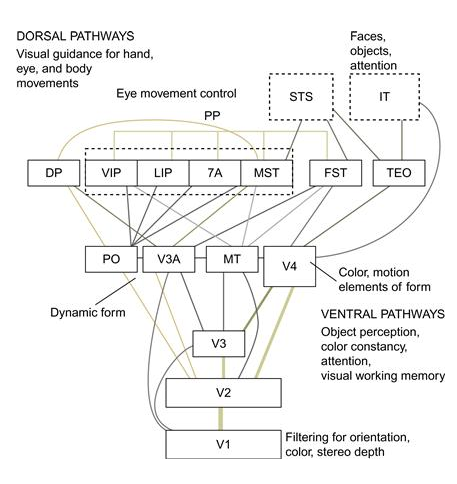
\includegraphics[width=0.4\textwidth]{brain.png}
%        \caption{Macaque monkey brain}
%    \end{figure}


\secttoc


Visualization is the application of vision research to problems of data
analysis. As visualization becomes more important, so does its scientific
understanding. Sensory and arbitrary symbols are split by fundamental
differences, but classification can be difficult. Consistent notation is most
important. This book assumes all humans have more or less the same visual
system.

\begin{mdframed}\begin{multicols}{2}
\subsection{Visualization}
        \begin{figure}[H]
            \centering
            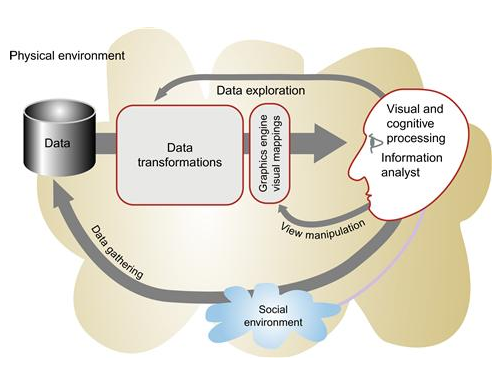
\includegraphics[width=0.3\textwidth]{stages.png}
            \caption{Stages of visualization}
        \end{figure}
\begin{compactdesc}
    \item[Visualization] A graphical representation of data or concepts. Old:
        constructing a visual image in the mind.
    \item[Benefits of visualization]:
        \begin{compactenum}
        \item Comprehend huge amounts of data
        \item Perception of unanticipated, emergent properties
        \item Problems with data become apparent
        \item Understanding of both large-scale and small-scale features
        \item Hypothesis formation is encouraged
        \end{compactenum}
    \item[Visualization stages] form feedback loops in the search for new
        information:
    \item[Data gathering] is the longest feedback loop.
    \item[Visualization] can be highly interactive

        \begin{figure}[H]
            \centering
            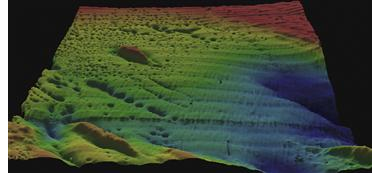
\includegraphics[width=0.25\textwidth]{pasamoquoddy_vis.png}
            \caption{Pasamoquoddy bay scans. A lot of data. Roll of the ship
            was not corrected for.}
        \end{figure}


\end{compactdesc}
\end{multicols}\end{mdframed}

\begin{mdframed}\begin{multicols}{2}
\subsection{Semiotics}

\begin{compactdesc}
\item[Semiotics] the study of making meaning. Signs, analogy, indication,
    designation, metaphor, symbol, communication.
\item[Counter-argument:] diagrams are arbitary, all symbols are learned thus
    one visualization is as good as another regardless of ease of perception.
\item[This debate] helps us decide where visualization science is useful and
    where we should consult a trained designer.
\item[Semiotics of graphics] dominated by non-rigorous philosophers. What is a
    visual language?
\item[Biggest threat] philosophers argue that truth is only so in the context
    of its creators' culture. Meaning is curated by culture. All representations
    have meaning to those trained/raised to know them.
\item[These arguments are rejected] we can have a new semiotics based on
    scientific evidence, not philosopher's claims.
\item[People can interpret] pictures without training clearly (2 studies). The
    outline of an object and the object itself excite similar neural processes.
\end{compactdesc}
\end{multicols}\end{mdframed}




\begin{mdframed}\begin{multicols}{2}
\subsection{Sensory vs Arbitrary}

\begin{compactdesc}
\item[Sensory] is defined here as the aspects of representation that are
    expressive due to the natural perceptual processing power of the brain.
    Full scientific methodology can be applied. Nearly universal.
\item[Arbitrary] is defined here as the aspects of representation that must
    be learned. Interpretive methodology needed.
\item[Example] circles in nearly all cultures represent a bounded region
\item[We reject the idea] that the visual system can adapt to any universe,
    and that our vision is intertwined with this planet.
\item[Many specialized] regions in our brain develop only for their single
    purpose, not a tabula rasa.
\item[Small adaptations] cats raised in a world of only vertical stripes
    develop an unusual number of vertical-edge detectors
\item[Macaque Monkey's] visual system: V1 (orientation, color, stereo depth)
    $\to$ V2 $\to$ V3 $\to$ V4 (Color, motion, elements of form) and other
    systems. Also: object perception, color constancy, attention, visual
    working memory.
\item[Sensory representations] work because they are well matched to the
    first stages of perception.
    \begin{compactenum}
    \item Understanding without training
    \item Resistance to alternate denotation
    \item Sensory immediacy
    \item Cross cultural validity
    \end{compactenum}
\item[Vision researchers and biologists] can test claims about sensory
    representation.
\item[Arbitrary codes] are socially constructured
    \begin{compactenum}
    \item Hard to learn
    \item Easy to forget
    \item Embedded in culture and applications
    \item Formally powerful, can be matched to rigorous languages
    \end{compactenum}
\item[Sensory and arbitary are intertwined] but the visualization designer must
    still be able to apply the science of visualization
\end{compactdesc}

        \begin{figure}[H]
            \centering
            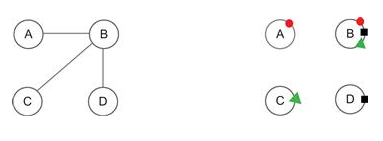
\includegraphics[width=0.3\textwidth]{graph_vis.png}
            \caption{Left visualization is easier to interpret}
        \end{figure}



\end{multicols}\end{mdframed}




\begin{mdframed}\begin{multicols}{2}
    \subsection{Gibson's Affordance theory}

\begin{compactdesc}
\item[Affordances] are possibilities for action that can be percevied
\item[Directly] seen, not inferred from sensory cues.
\item[Action-based] perception!
\item[We do not perceive] points of light and go up from there, our visual
    system works from top to bottom.
\item[Three problems]:
    \begin{compactenum}
    \item Computer graphics are very indirect, detached from the way we
        interact with them
    \item No clear physical affordances in any graphical user interface.
        Buttons are arbitrary
    \item Gibson rejected visual mechanisms. Mistake. Color perception is an inborn
        trait, it is actually a thoroughly studied system, and it is entirely
        bottom-up.
    \end{compactenum}
\end{compactdesc}
    \subsection{A model of perceptual processing}
\begin{compactdesc}
\item[Stage 1: Parallel processing, low-level properties] primitive, specialized
    and fast. Bottom-up, visual salience. If information must be understood
    quickly, here is where optimizations are needed.
\item[Stage 2: Pattern Perception] Rapid processes divide the field into
    regions and simple patterns like contours and regions of shared
    color/texture. Motion. Flexible. Deals with the massive amount of data
    from stage 1 and tunes queries using the higher-level process of attention.
    Slower, serial. One to three objects can be held for a second or two.
\item[Stage 3: Visual working meory] highest level. Sequence of visual
    queries. Only a few objects held at a time. Constructed from the lower
    levels.
\item[Attention] The top-down signal that consolidates and enhances the jobs
    of the visual system. Multifaceted, pervasive.
\end{compactdesc}
\end{multicols}\end{mdframed}




\begin{mdframed}\begin{multicols}{2}
\subsection{Costs and Benefits of Visualization}

\begin{compactdesc}
\item[Must measure value] in some way to optimize a system. Workers will work
    easier, less stress. A scientific discovery could be made.
\item[Cost for user:] time to learn
\item[Benefit for user:] improved cognitive workload
\item[Cost for dev:] time to develop visualization, cost to market,
    manufacture, service
\item[Benefits for dev:] units sold, revenue
\end{compactdesc}

\subsection{Types of data}
\begin{compactenum}
\item entities, relationships, attributes
\item dimensionality: 1,2,3 and up
\item types of numbers
\item uncertainty
\item operations such as arithmetic, merging, removing
\item metadata: data about data, who/what, transforms and uncertainty
\end{compactenum}


\end{multicols}\end{mdframed}

